\documentclass[12pt,letterpaper, onecolumn]{exam}
\usepackage{amsmath}
\usepackage{amssymb}
\usepackage[lmargin=71pt, tmargin=1.2in]{geometry}  %For centering solution box
\lhead{Samuel Molero\\}
\rhead{Section: 501\\}
\usepackage{subcaption}
\usepackage{graphicx}
% \chead{\hline} % Un-comment to draw line below header
\thispagestyle{empty}   %For removing header/footer from page 1

\begin{document}
\begingroup  
    \centering
    \LARGE STATS 211\\
    \LARGE Homework 1 \\[0.5em]
    \large \today\\[0.5em]
    \large Samuel Molero\par
    \large samueljosemolero@tamu.edu\par
    \large Section: 501\par
\endgroup
\rule{\textwidth}{0.4pt}
\pointsdroppedatright   %Self-explanatory
\printanswers
\renewcommand{\solutiontitle}{\noindent\textbf{Ans:}\enspace}   %Replace "Ans:" with starting keyword in solution box

\begin{questions}

    \question Q1? \\
    \begin{parts}
        \part Construct the (t, y) and (t, log(y)) scatter plot. Which scatter plot suggests a linear relationship?\\
            \begin{solution}
            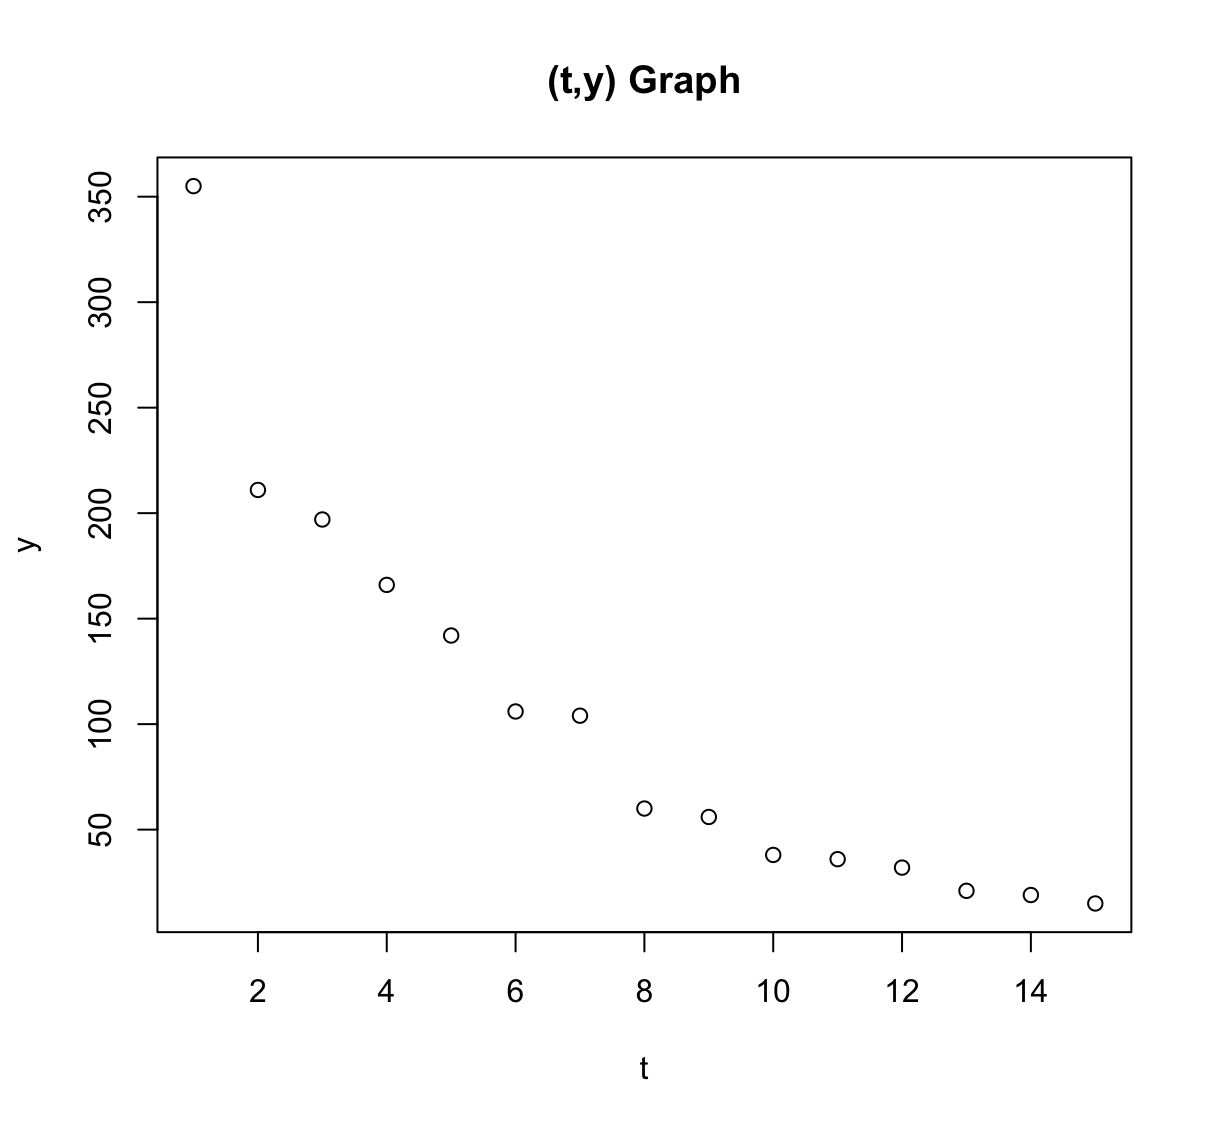
\includegraphics[width=0.4\textwidth]{Homeworks/yGraph.png} 
            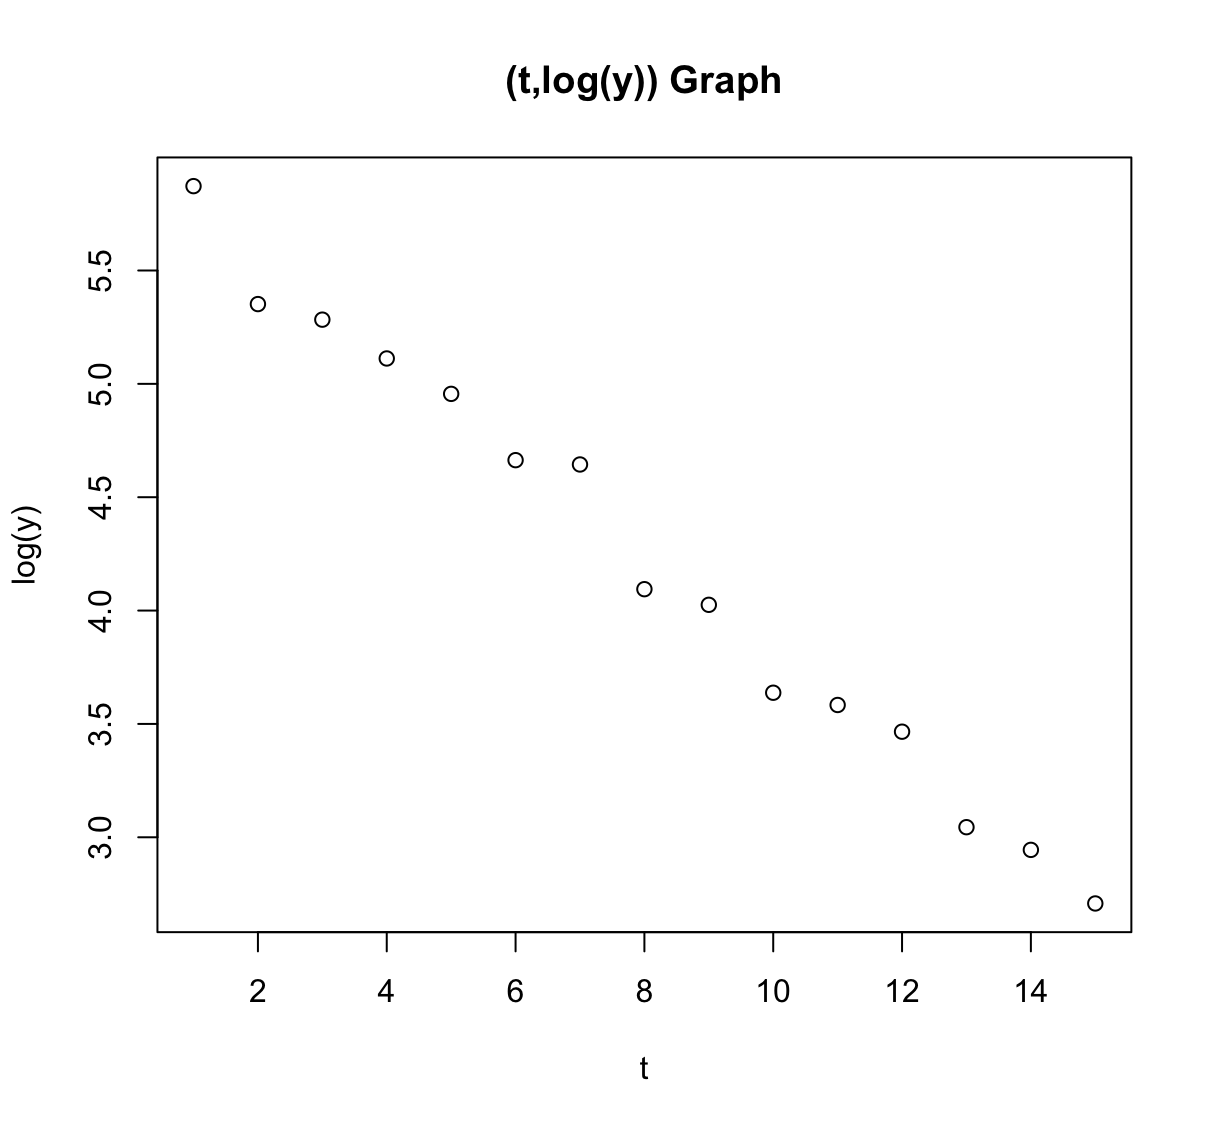
\includegraphics[width=0.4\textwidth]{Homeworks/Log(y)Graph.png}
             
            Scatter plot $(t,log(y))$ presents a linear relation.
            \end{solution}
        \part Construct a predictive equation for the bacteria count Y at time t.
        \begin{solution}
            \begin{verbatim}
                # R code snippet
                # lm_fit <- lm(y_log~t)
                # summary(lm_fit)
            \end{verbatim}
            Using the command above will provide both the intercept and slope for the linear regression equation using the log form values of Y. Which results in the following equation:\\
            \center
            $ log(\hat{y})  = 5.9732 -0.2184t$\\
            Solving for the predictive model for bacteria count Y at time t results in:\\
            $y = e^{5.9732 -0.2184t}$
        \end{solution}
        
    \end{parts}
    
    
    \question Q2?
    
    \begin{solution}
            
        \begin{parts}
            \part  
            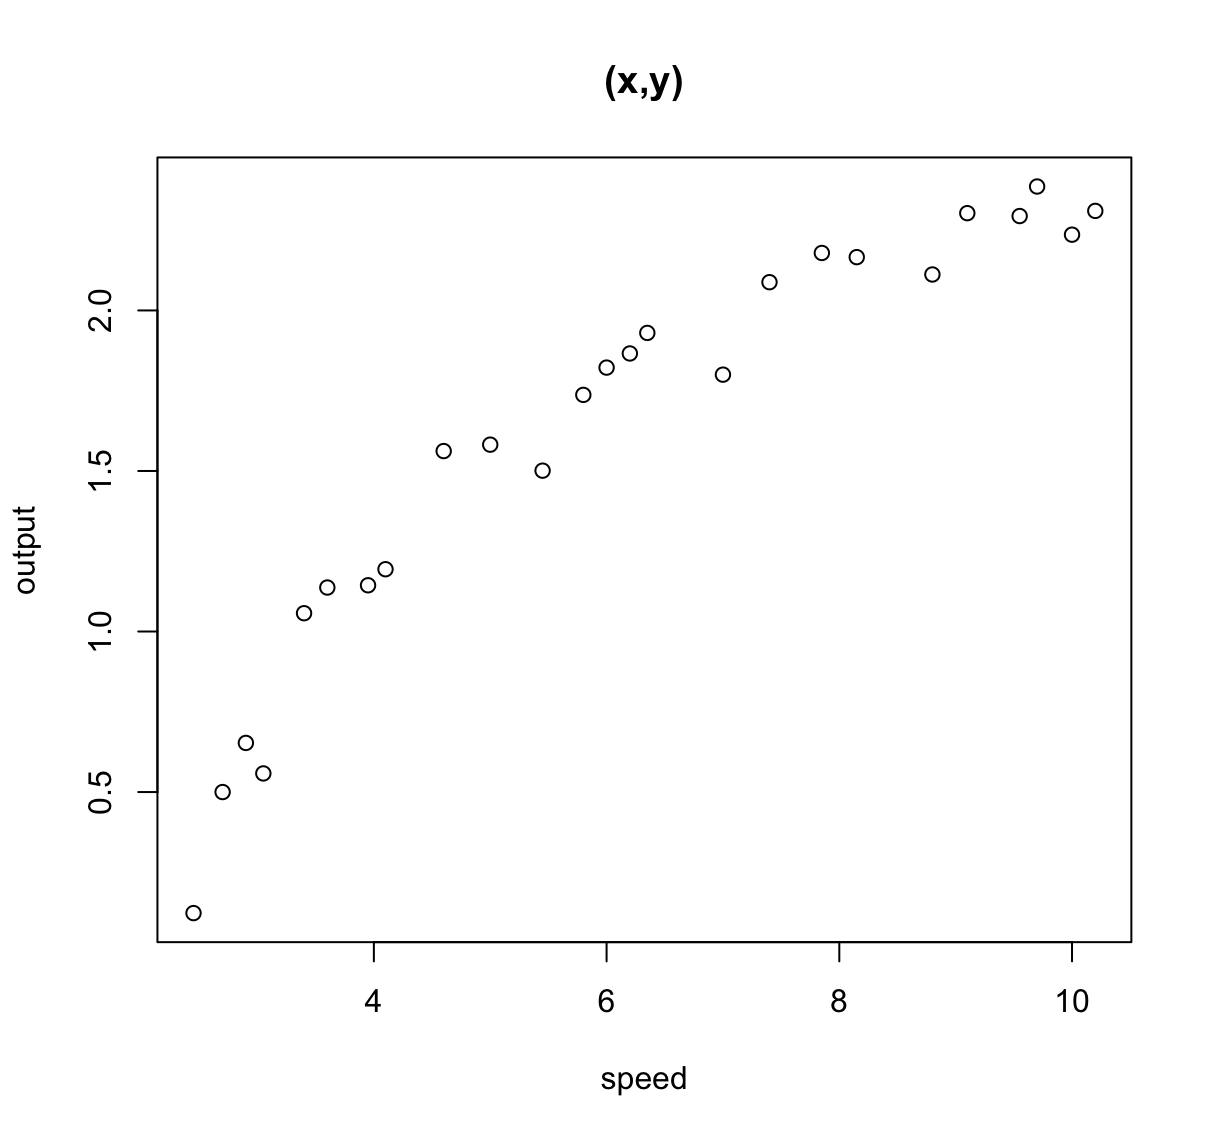
\includegraphics[width=0.48\textwidth]{Homeworks/(x,y).png}
            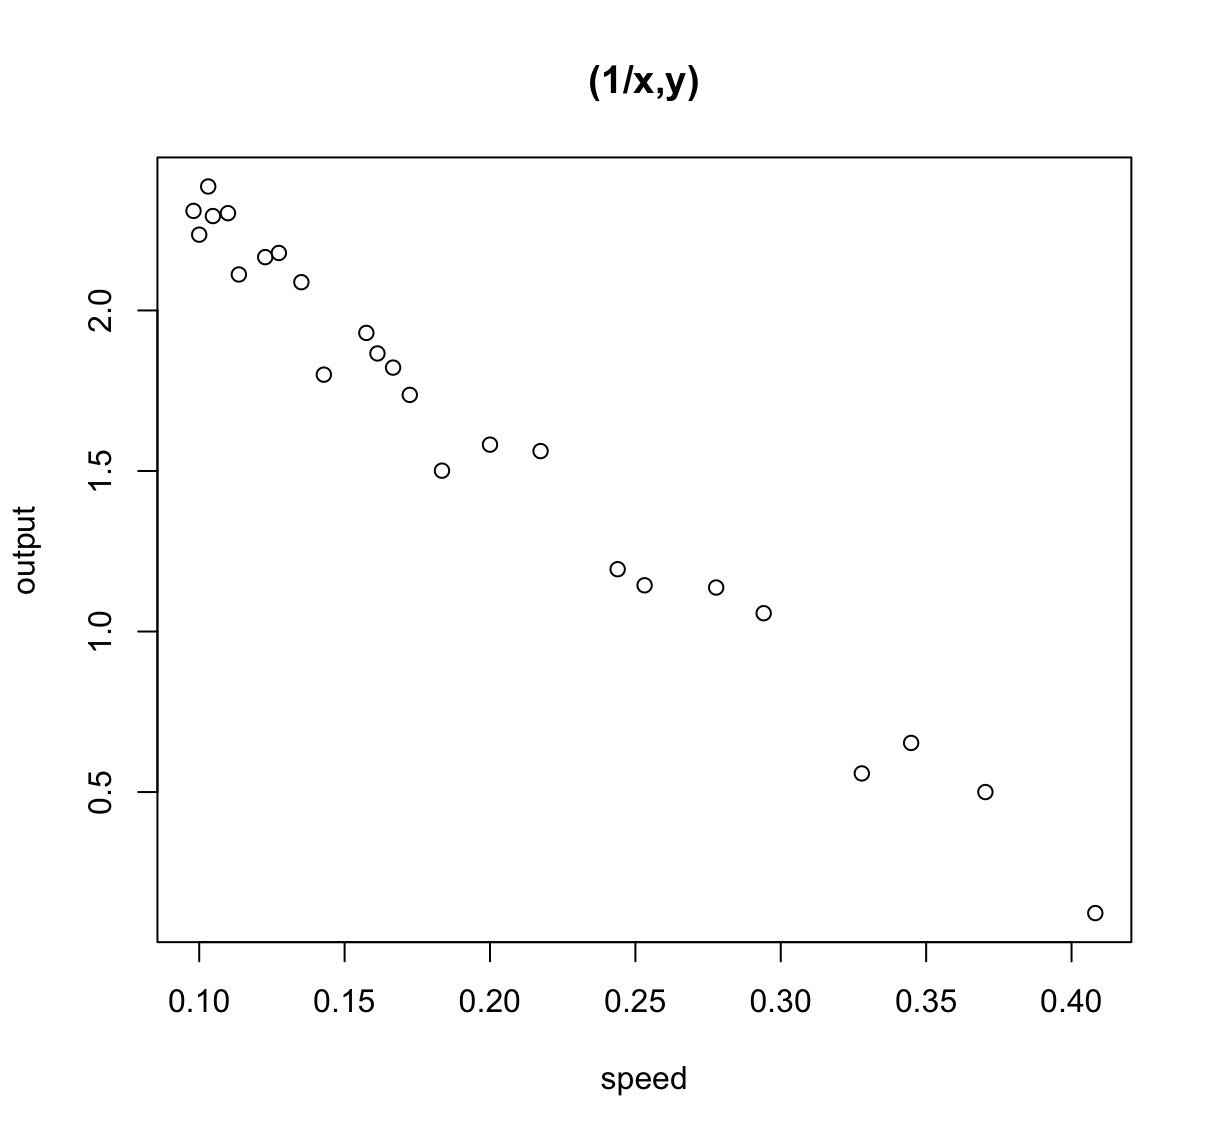
\includegraphics[width=0.48\textwidth]{Homeworks/(1:x,y).png}
            Scatter plot $(1/x,y)$ suggest a linear relation.
            \part 
            \begin{verbatim}
                #lim_fit <-lm(output~speed2)
                #summary(lim_fit)
            \end{verbatim}
                Using the transformed data from the second graph and the commands above, the linear regression is the following: $\hat{y} = 2.9789 -6.935/x$\\
            
            \part 
            Using Wind Speed of 8: $\hat{y} = 2.9789 -6.935/(8) = 2.1120$\\

            \part
            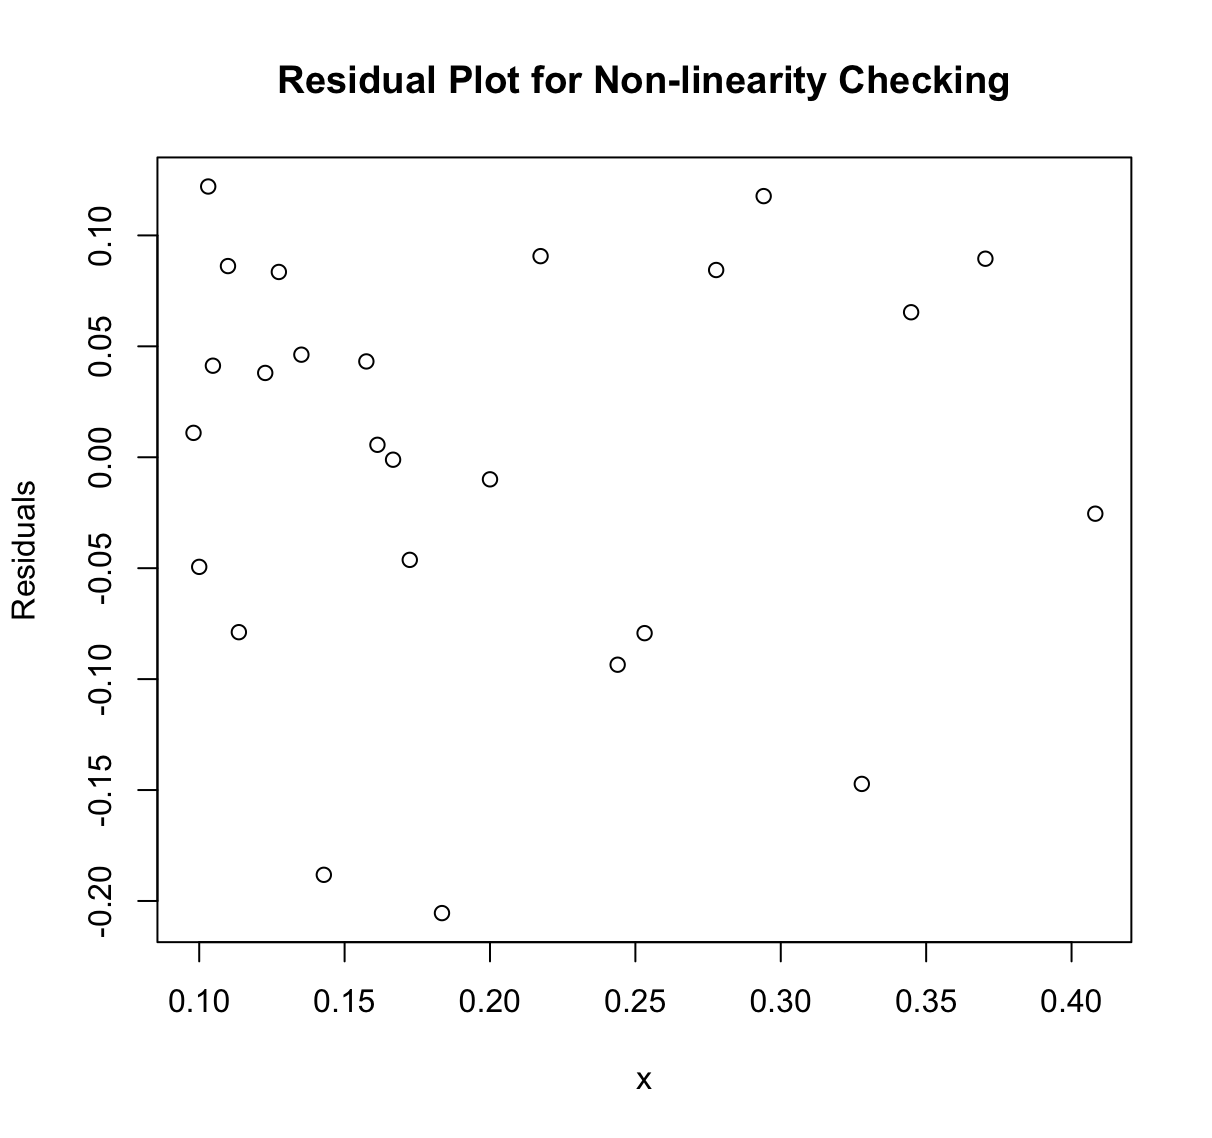
\includegraphics[width=0.48\textwidth]{Homeworks/First.png}
            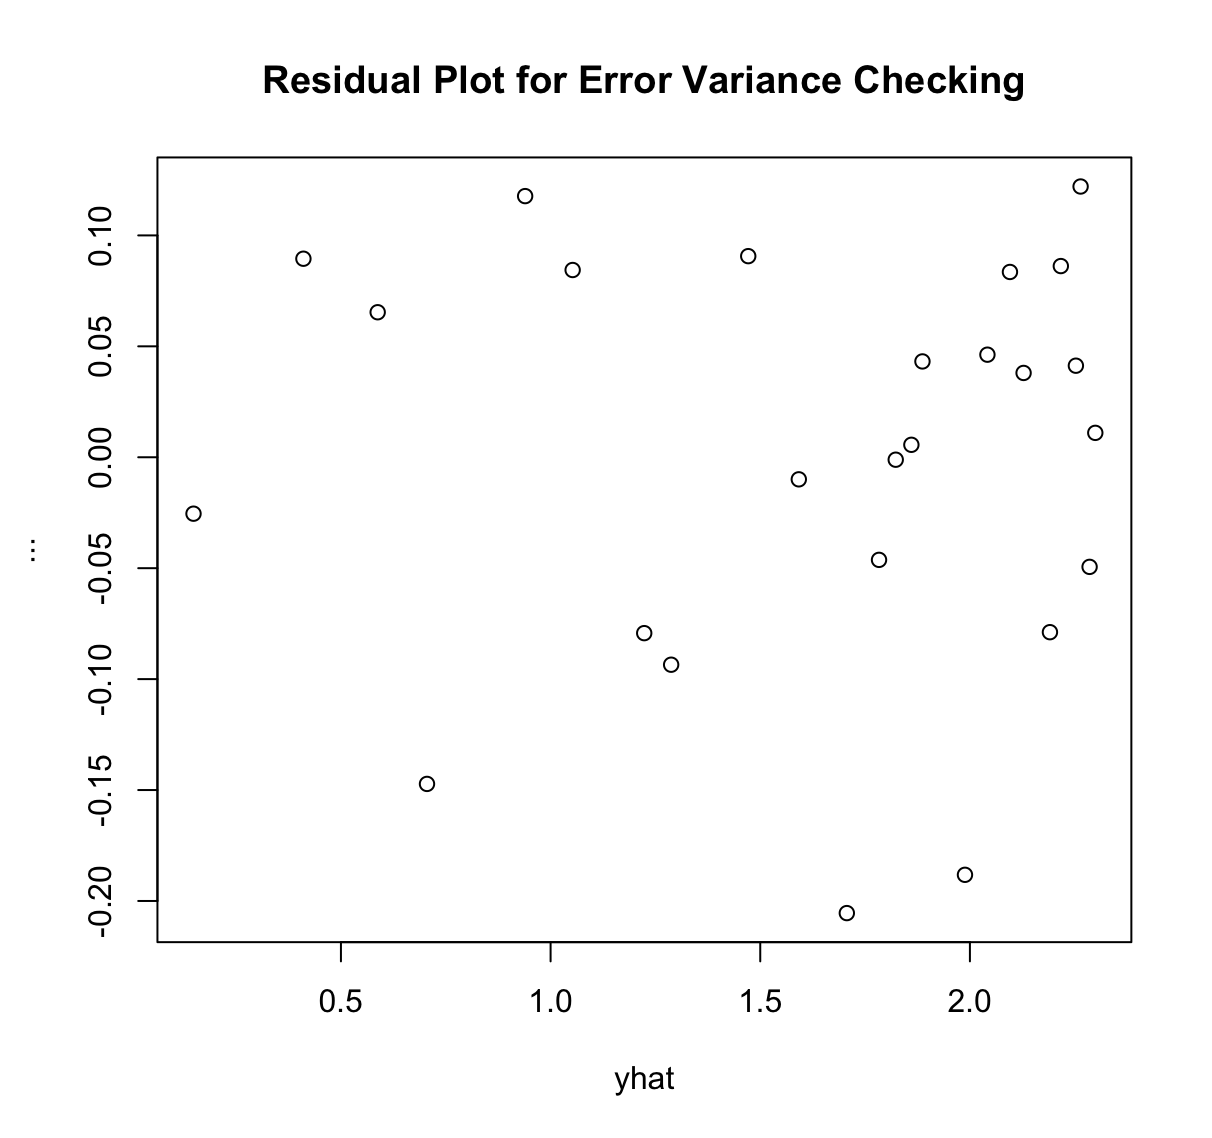
\includegraphics[width=0.48\textwidth]{Homeworks/Second.png}
            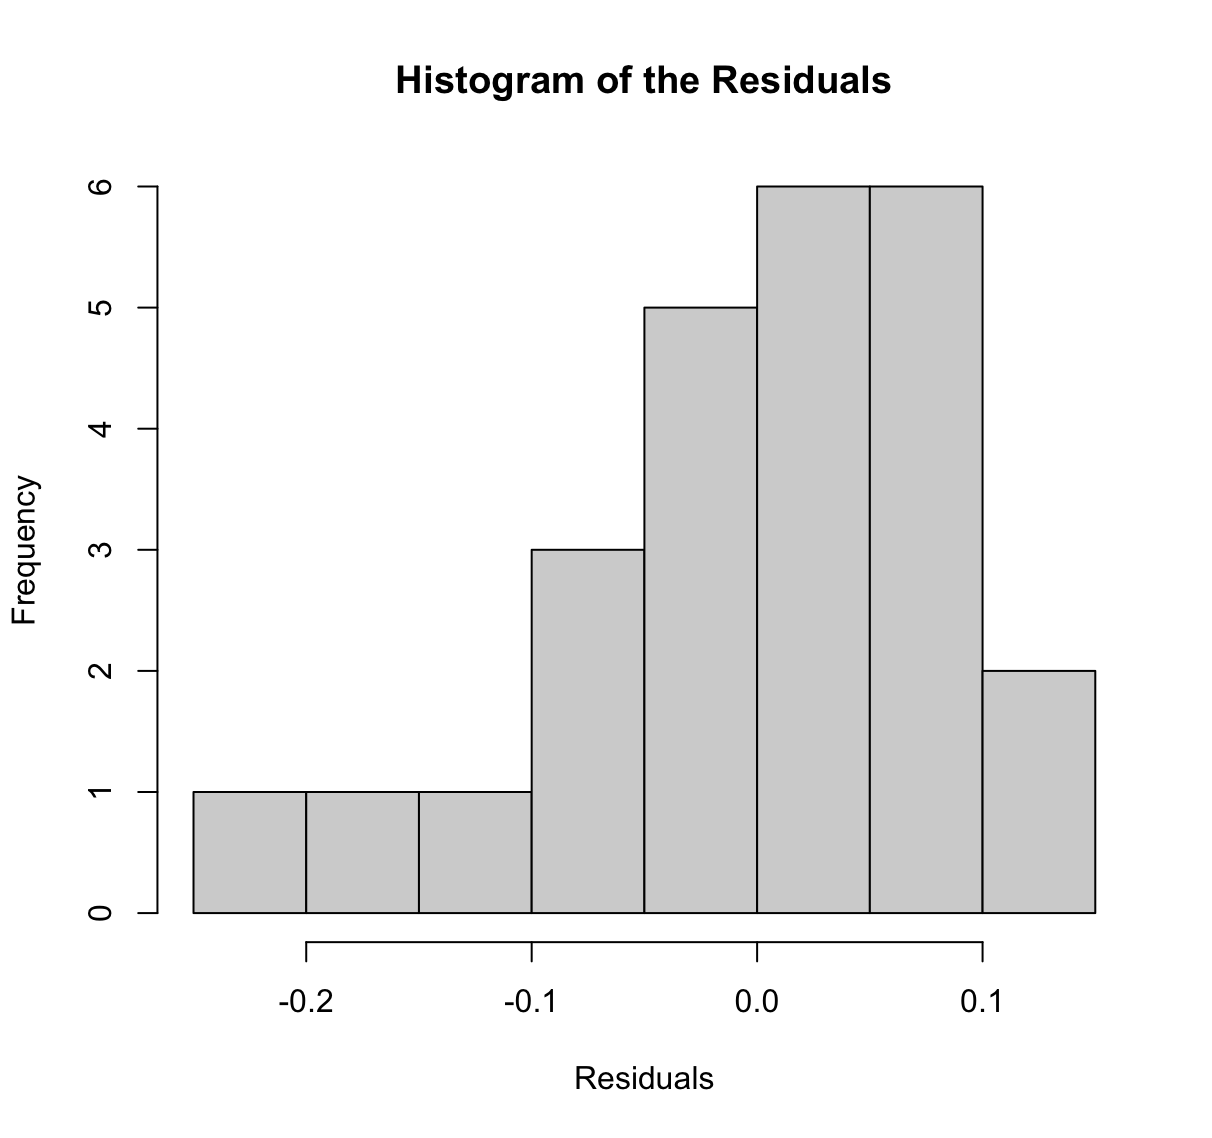
\includegraphics[width=0.48\textwidth]{Homeworks/Third.png}
            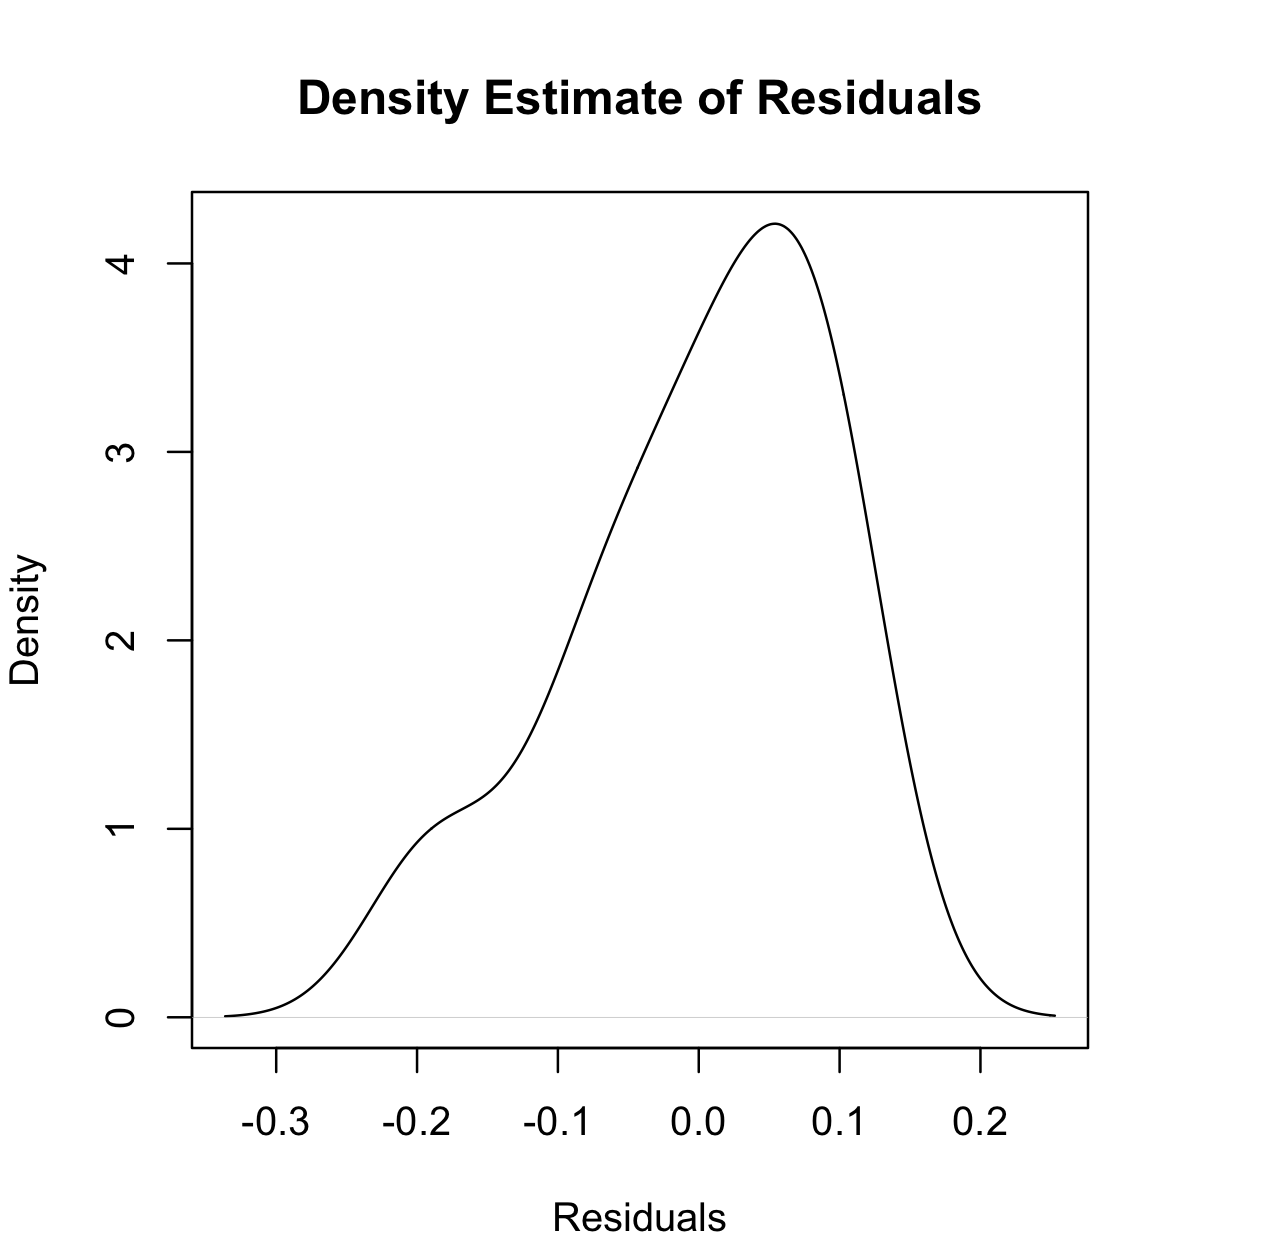
\includegraphics[width=0.48\textwidth]{Homeworks/Fourth.png}
            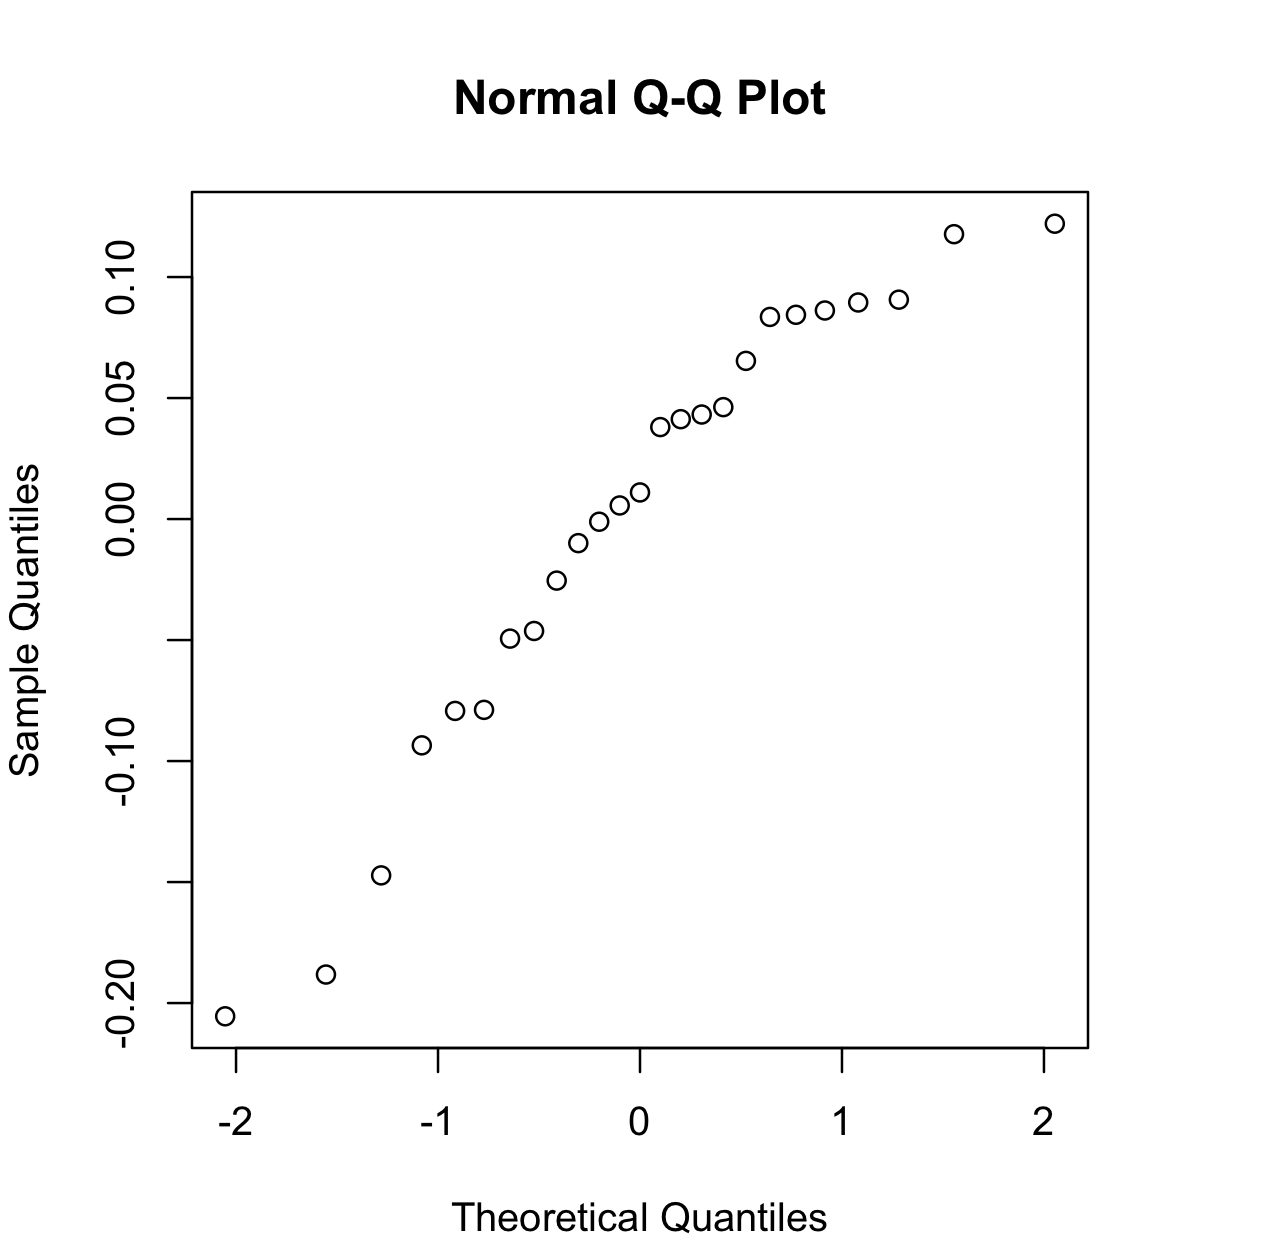
\includegraphics[width=0.48\textwidth]{Homeworks/Fifth.png}\\
            \newpage
            
            \part The $R^{2}$ obtained equals 0.9800, meaning that 98\%\ of the variation in wind speed's output is explained by linear regression. \\

            \part 
            \begin{verbatim}
                # confint(lim_fit, level=0.99)
            \end{verbatim}
            $\beta_1 = [-7.514076 -6.355019]$, there is 99\%\ confidence that the true slope lies between the given values. 
            

            \part 
            \begin{verbatim}
            predict(lm(output~speed2), data.frame(speed=3.2),
            interval ="confidence", level=0.95)
            \end{verbatim}
            Given that thewind speedd is 3.2, there is 95\%\ confidence that the true value lies within the interval $[0.74911,0.87451]$

            \part 
            \begin{verbatim}
                predict(lim_fit, data.frame(speed=9.05), 
                interval ="prediction", level=0.95)
            \end{verbatim}
            Given that the particular speed at a specific windmill is 9.05, the 95\%\ prediction interval for the output lies within the interval $[2.0105,2.4147]$
            
        
        \end{parts}
        
    \end{solution}

    
\end{questions}
\end{document}